\documentclass[table]{beamer}
%[]中可以使用draft、handout、screen、transparency、trancompress、compress等参数

%指定beamer的模式与主题
\mode<presentation>
{
  \usetheme{Madrid}
%\usetheme{Boadilla}
%\usecolortheme{default}
%\usecolortheme{orchid}
%\usecolortheme{whale}
%\usefonttheme{professionalfonts}
}

%\usetheme{Madrid}
%这里还可以选择别的主题:Bergen, Boadilla, Madrid, AnnArbor, CambridgeUS, Pittsburgh, Rochester, Warsaw, ...
%有导航栏的Antibes, JuanLesPins, Montpellier, ...
%有内容的Berkeley, PaloAlto, Goettingen, Marburg, Hannover, ...
%有最小导航栏的Berlin, Ilmenau, Dresden, Darmstadt, Frankfurt, Singapore, Szeged, ...
%有章和节表单的Copenhagen, Luebeck, Malmoe, Warsaw, ...

%\usecolortheme{default}
%设置内部颜色主题(这些主题一般改变block里的颜色);这个主题一般选择动物来命名
%这里还可以选择别的颜色主题,如默认的和有特别目的的颜色主题default,structure,sidebartab,全颜色主题albatross,beetle,crane,dove,fly,seagull,wolverine,beaver

%\usecolortheme{orchid}
%设置外部颜色主题(这些主题一般改变title里的颜色);这个主题一般选择植物来命名
%这里还可以选择别的颜色主题,如默认的和有特别目的的颜色主题lily,orchid,rose

%\usecolortheme{whale}
%设置字体主题;这个主题一般选择海洋动物来命名
%这里还可以选择别的颜色主题,如默认的和有特别目的的颜色主题whale,seahorse,dolphin

%\usefonttheme{professionalfonts}
%类似的还可以定义structurebold,structuresmallcapsserif,professionalfonts


% 控制 beamer 的风格,可以根据自己的爱好修改
%\usepackage{beamerthemesplit} %使用 split 风格
%\usepackage{beamerthemeshadow} %使用 shadow 风格
%\usepackage[width=2cm,dark,tab]{beamerthemesidebar}

%插入音标
\usepackage{tipa}
\AtBeginDocument{
  \renewcommand\textipa{\fontencoding{T3}\selectfont}
}
\AtBeginDocument{
  \renewcommand\textipa[2][r]{{\fontfamily{cm#1}\tipaencoding #2}}
}
\renewenvironment{IPA}[1][r]
 {\fontfamily{cm#1}\tipaencoding}
 {}

% 设定英文字体
%\usepackage{fontspec}
\usepackage[no-math]{fontspec}
\setmainfont{Times New Roman}
\setsansfont{Arial}
\setmonofont{Courier New}

% 设定中文字体
\usepackage[BoldFont,SlantFont,CJKchecksingle,CJKnumber]{xeCJK}
%\setCJKmainfont[BoldFont={Adobe Heiti Std},ItalicFont={Adobe Kaiti Std}]{Adobe Song Std}
\setCJKmainfont[BoldFont={Adobe Heiti Std},ItalicFont={Adobe Kaiti Std}]{WenQuanYi Micro Hei}
\setCJKsansfont{Adobe Heiti Std}
\setCJKmonofont{Adobe Fangsong Std}
\punctstyle{hangmobanjiao}

\defaultfontfeatures{Mapping=tex-text}
\usepackage{xunicode}
\usepackage{xltxtra}

\XeTeXlinebreaklocale "zh"
\XeTeXlinebreakskip = 0pt plus 1pt minus 0.1pt

\usepackage{setspace}
\usepackage{colortbl,xcolor}
\usepackage{hyperref}
%\hypersetup{xetex,bookmarksnumbered=true,bookmarksopen=true,pdfborder=1,breaklinks,colorlinks,linkcolor=blue,filecolor=black,urlcolor=cyan,citecolor=green}
\hypersetup{xetex,bookmarksnumbered=true,bookmarksopen=true,pdfborder=1,breaklinks,colorlinks,linkcolor=cyan,filecolor=black,urlcolor=blue,citecolor=green}

% 插入图片
\usepackage{graphicx}
\graphicspath{{figures/}}
% 图文混排
\usepackage{picins}
\usepackage{floatflt}

% 可能用到的包
\usepackage{amsmath,amssymb}
%插入多媒体
%\usepackage{media9}
%\usepackage{movie15}
\usepackage{multimedia}
\usepackage{multicol}
\usepackage{multirow}

% 定义一些自选的模板,包括背景、图标、导航条和页脚等,修改要慎重
% 设置背景渐变由10%的红变成10%的结构颜色
%\beamertemplateshadingbackground{red!10}{structure!10}
%\beamertemplatesolidbackgroundcolor{white!90!blue}
% 使所有隐藏的文本完全透明、动态,而且动态的范围很小
\beamertemplatetransparentcovereddynamic
% 使itemize环境中变成小球,这是一种视觉效果
\beamertemplateballitem
% 为所有已编号的部分设置一个章节目录,并且编号显示成小球
\beamertemplatenumberedballsectiontoc
% 将每一页的要素的要素名设成加粗字体
\beamertemplateboldpartpage

% item逐步显示时,使已经出现的item、正在显示的item、将要出现的item呈现不同颜色
\def\hilite<#1>{
 \temporal<#1>{\color{gray}}{\color{blue}}
    {\color{blue!25}}
}

\renewcommand{\today}{\number\year 年 \number\month 月 \number\day 日}

%五角星
\usepackage{MnSymbol}

%去除图表标题中的figure等
\usepackage{caption}
\captionsetup{labelformat=empty,labelsep=none}

\usepackage{tabu}
\usepackage{multirow}
%表格自动换行
\usepackage{tabularx} 

% 千分号
%\usepackage{textcomp}

%罗马数字
\makeatletter
\newcommand{\rmnum}[1]{\romannumeral #1}
\newcommand{\Rmnum}[1]{\expandafter\@slowromancap\romannumeral #1@}
\makeatother

%分栏
\usepackage{multicol}

%\usepackage{enumitem}
%\usepackage{enumerate}

%键盘
\usepackage{keystroke}

%插入源代码
\usepackage{listings}
\lstset{
  language=bash,                  % 程序语言名称:TeX, Perl, R, sh, bash, Awk
  basicstyle=\normalsize\tt,      %\tt指monospace字体族,程序源代码使用此族字体表示更加美观
  numbers=left,                   % 行号位置(左侧)
  numberstyle=\small,             % 行号字体的字号
  stepnumber=1,                   % 行号的显示步长
  numbersep=5pt,                  % 行号与代码间距
  backgroundcolor=\color{white},  % 背景色;需要 \usepackage{color}
  showspaces=false,               % 不显示空格
  showstringspaces=false,         % 不显示代码字符串中的空格标记
  showtabs=false,                 % 不显示 TAB
  tabsize=4, 
  frame=shadowbox,                % 把代码用带有阴影的框圈起来
  captionpos=b,                   % 标题位置
  breaklines=true,                % 对过长的代码自动断行
  breakatwhitespace=false,        % 断行只在空格处
  extendedchars=false,            % 解决代码跨页时,章节标题,页眉等汉字不显示的问题
  %escapeinside={\%*}{*},         % 跳脱字符,添加注释,暂时离开 listings 
  %escapeinside=``,
  commentstyle=\color{red!50!green!50!blue!50}\tt,  %浅灰色的注释
  rulesepcolor=\color{red!20!green!20!blue!20},     %代码块边框为淡青色
  keywordstyle=\color{blue!70}\bfseries\tt,         %代码关键字的颜色为蓝色,粗体
  identifierstyle=\tt,
  stringstyle=\tt,                % 代码字符串的特殊格式
  keepspaces=true,
  breakindent=1em,
  %breakindent=22pt,
  %breakindent=4em,
  breakautoindent=true,
  flexiblecolumns=true,
  aboveskip=1em,                  %代码块边框
  xleftmargin=2em,
  xrightmargin=2em
}

%\setbeamercolor{alerted text}{fg=magenta}
\setbeamercolor{bgcolor}{fg=yellow,bg=cyan}
%\setbeamercolor{itemize/enumerate body}{fg=green}

\begin{document}

%\includeonlyframes{current}

\logo{
\includegraphics[height=0.08\textwidth]{tijmu.png}}

% 在每个Section前都会加入的Frame
\AtBeginSection[]
{
  \begin{frame}<beamer>
    %\frametitle{Outline}
    \frametitle{教学提纲}
    \setcounter{tocdepth}{3}
    \begin{multicols}{2}
      \tableofcontents[currentsection,currentsubsection]
      %\tableofcontents[currentsection]
    \end{multicols}
  \end{frame}
}
% 在每个Subsection前都会加入的Frame
\AtBeginSubsection[]
{
  \begin{frame}<beamer>
%%\begin{frame}<handout:0>
%% handout:0 表示只在手稿中出现
    \frametitle{教学提纲}
    \setcounter{tocdepth}{3}
    \begin{multicols}{2}
    \tableofcontents[currentsection,currentsubsection]
    \end{multicols}
%% 显示在目录中加亮的当前章节
  \end{frame}
}

% 为当前幻灯片设置背景
%{
%\usebackgroundtemplate{
%\vbox to \paperheight{\vfil\hbox to
%\paperwidth{\hfil
\includegraphics[width=2in]{tijmu_charcoal.png}\hfil}\vfil}
%}
\begin{frame}[plain]
  \begin{center}
    {\Huge Linux系统概论\\}
    \vspace{1cm}
    {\LARGE 天津医科大学\\}
    %\vspace{0.2cm}
    {\LARGE 生物医学工程与技术学院\\}
    \vspace{1cm}
    {\large 2017-2018学年下学期(春)\\ 2016级生信班}
  \end{center}
\end{frame}
%}



%\includeonlyframes{current}

\title[文件系统]{第三章\quad 文件系统}
\author[Yixf]{伊现富(Yi Xianfu)}
\institute[TIJMU]{天津医科大学(TIJMU)\\ 生物医学工程与技术学院}
\date{2016年3月}


\begin{frame}
  \titlepage
\end{frame}

\begin{frame}[plain,label=current]
  \frametitle{教学提纲}
  \setcounter{tocdepth}{3}
  \begin{multicols}{2}
    \tableofcontents
  \end{multicols}
\end{frame}

\section{插曲}
\begin{frame}[fragile]
  \frametitle{\textcolor{gray}{插曲 | 抽签}}
  \begin{block}{使用学生名单}
    \begin{itemize}
      \item \verb=shuf -n 10 students.list=
      \item \verb=sort -R students.list | head=
    \end{itemize}
  \end{block}
  \pause
  \begin{block}{通过学号}
    \begin{itemize}
      \item 简单的学号数字(剔除没有的学号):\verb=seq 33 | grep -v "^8$" | grep -v "^11$" | shuf -n 10=
      \item 添加学号前缀:\verb=seq -w 33 | grep -v "^8$" | nl -s "20130521" | cut -c7- | shuf -n 10=
      \item 添加学号前缀:\verb=seq -w 33 | grep -v "^8$" | sed "s/^/20130521/" | shuf -n 10=
    \end{itemize}
  \end{block}
\end{frame}

\begin{frame}[fragile]
  \frametitle{\textcolor{gray}{插曲 | 抽奖}}
  %\begin{block}{使用观众名单}
    \begin{enumerate}
      \item 抽取三等奖:\verb=shuf -n 10 all.list > level3.list=
      \item 删除中三等奖观众:\verb=grep -f level3.list -v all.list > all-3.list=
      \item 抽取二等奖:\verb=shuf -n 3 all-3.list > level2.list=
      \item 删除中二等奖观众:\verb=grep -f level2.list -v all-3.list > all-3-2.list=
      \item 抽取一等奖:\verb=shuf -n 1 all-3-2.list > level1.list=
      \item 未中奖观众:\verb=grep -f level1.list -v all-3-2.list > all-3-2-1.list=
    \end{enumerate}
  %\end{block}
  \pause
  \begin{block}{【课外作业】编写shell脚本}
    \begin{itemize}
      \item 随意指定中奖人数
      \item 自动删除中奖观众
      \item 处理缺席中奖观众
      \item ……
    \end{itemize}
  \end{block}
\end{frame}

\section{引言}
\begin{frame}
  \frametitle{文件系统 | 引言 | 文件系统}
\begin{block}{操作系统 vs. 文件系统}
\begin{itemize}
  \item 终端用户 $\Longleftrightarrow$ 操作系统 $\Longleftrightarrow$ 计算机硬件
  \item 终端用户 $\Longleftrightarrow$ 文件系统 $\Longleftrightarrow$ 硬盘等存储设备
\end{itemize}
\end{block}
\pause
  \footnotesize{
  计算机的\textbf{文件系统(File system)}是一种存储和组织计算机数据的方法,它使得对其访问和查找变得容易,文件系统使用\textbf{文件}和\textbf{树形目录}的抽象逻辑概念代替了硬盘和光盘等物理设备使用数据块的概念,用户使用文件系统来保存数据不必关心数据实际保存在硬盘(或者光盘)的地址为多少的数据块上,只需要记住这个文件的所属目录和文件名。在写入新数据之前,用户不必关心硬盘上的那个块地址有没有被使用,硬盘上的存储空间管理(分配和释放)功能由文件系统自动完成,用户只需要记住数据被写入到了哪个文件中。\\
  \vspace{0.1cm}
严格地说,文件系统是一套实现了数据的存储、分级组织、访问和获取等操作的抽象数据类型(Abstract data type)。\\
  \vspace{0.1cm}
文件系统通常使用硬盘和光盘这样的存储设备,并维护文件在设备中的物理位置。但是,实际上文件系统也可能仅仅是一种访问数据的界面而已,实际的数据是通过网络协议(如NFS、SMB、9P等)提供的或者存储在内存中,甚至可能根本没有对应的文件(如proc文件系统)。
}
\end{frame}

\begin{frame}
  \frametitle{文件系统 | 引言 | 文件系统的类型}
  \begin{enumerate}
    \item<1-> 面向磁盘的文件系统(本地的文件系统):位于硬盘、移动硬盘、光盘、U盘或其他设备上的实际可访问的文件系统。
      \begin{itemize}
        \item<4-> FAT(File Allocation Table,文件分配表):Windows
        \item<4-> NTFS(New Technology File System,新技术文件系统):Windows
	\item<4-> \alert{EXT4}(Extended Filesystem 4,扩展文件系统4):Linux
        \item<4-> Btrfs(B-Tree File System):Linux
        \item<4-> XFS(X File System):Linux
	\item<4-> \alert{ISO9660}:CD-ROM
        \item<4-> UFS(Unix File System,Unix文件系统):Unix
      \end{itemize}
    \item<2-> 面向网络的文件系统(基于网络的文件系统):可以远程访问的文件系统。
      \begin{itemize}
        \item<5-> NFS(Network File System,网络文件系统)
        \item<5-> Samba(SMB/CIFS)
      \end{itemize}
    \item<3-> 专用的或虚拟的文件系统:没有实际驻留在磁盘上的文件系统。
      \begin{itemize}
        \item<6-> TMPFS(临时文件系统)
        \item<6-> PROCFS(Process File System,进程文件系统)
      \end{itemize}
  \end{enumerate}
\end{frame}

\section{文件系统基础}
\subsection{文件系统和分区}
\begin{frame}
  \frametitle{文件系统 | 基础 | 文件系统和分区}
  \begin{block}{文件系统和分区}
    \begin{itemize}
      \item 分区是信息的容器,包含整个硬盘或硬盘的一部分
      \item 文件系统是多个文件的逻辑集合,位于分区或磁盘上
      \item 一个分区通常只包含一个文件系统
    \end{itemize}
  \end{block}
  \begin{figure}
    \centering
    \visible<2>{ 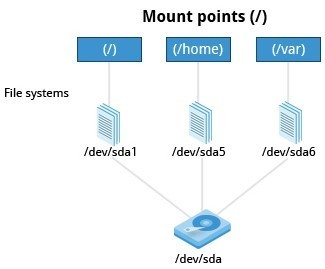
\includegraphics[width=6cm]{c3.partition.10.jpg} }
  \end{figure}
\end{frame}

\begin{frame}
  \frametitle{文件系统 | 基础 | 文件系统和分区}
  \begin{figure}
    \centering
    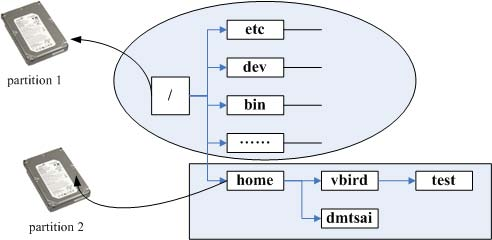
\includegraphics[width=8cm]{c3.partition.01.png}\\
    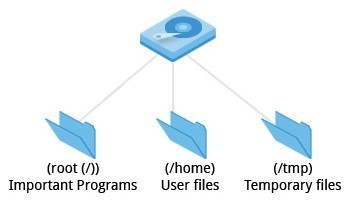
\includegraphics[width=6cm]{c3.partition.11.jpg}
  \end{figure}
\end{frame}

\subsection{目录结构}
\begin{frame}
  \frametitle{文件系统 | 基础 | \alert{目录结构}}
  \begin{figure}
    \centering
    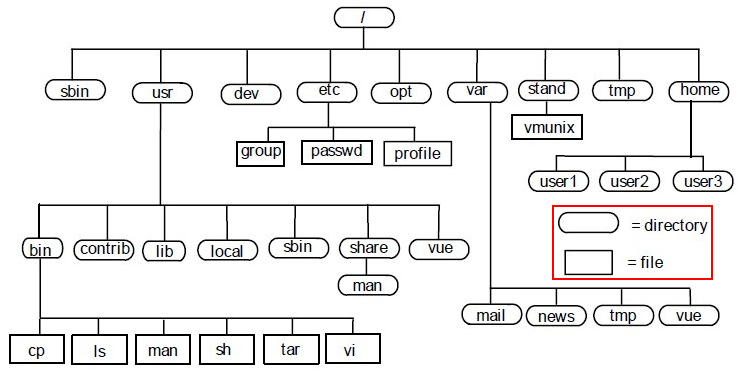
\includegraphics[width=9.5cm]{c3.filesystem.11.png}
  \end{figure}
  \pause
  \vspace{-0.3cm}
  %\begin{block}{Linux的目录结构}
    %\begin{itemize}[<+-|alert@+>]
    \begin{itemize}[<+->]
      \item Everything is a file.(一切皆文件。)
      \item 使用自顶而下的分层结构来组织文件
      \item 每个文件和目录都是从根目录(/)(Root Directory)开始的
      \item 文件和目录名的大小写是有区别的
      \item 定位文件:(根)目录$\Rightarrow$子目录$\Rightarrow$ \ldots $\Rightarrow$文件
    \end{itemize}
  %\end{block}
  %\begin{figure}
    %\centering
    %\vspace{-0.2cm}
    %\visible<6>{ 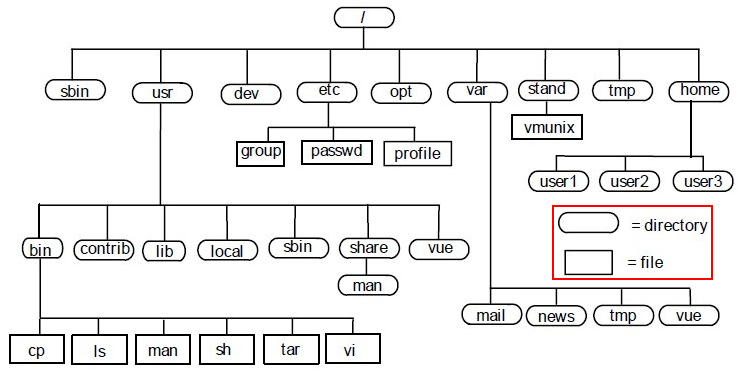
\includegraphics[width=9.5cm]{c3.filesystem.11.png} }
    %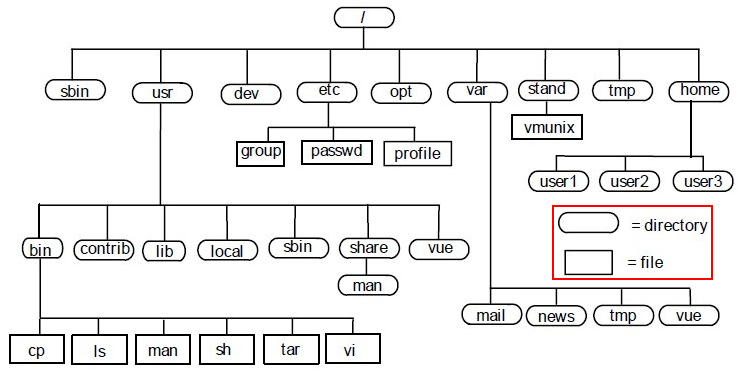
\includegraphics[width=9.5cm]{c3.filesystem.11.png}
  %\end{figure}
\end{frame}

\begin{frame}
  \frametitle{文件系统 | 基础 | \alert{目录结构}}
  \begin{figure}
    \centering
    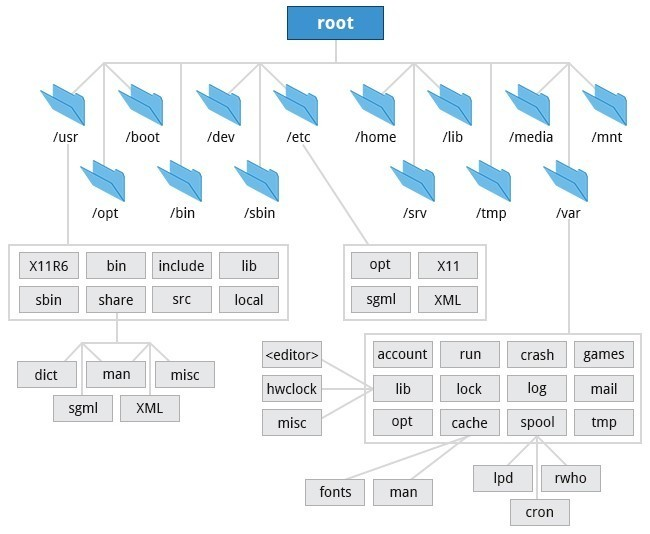
\includegraphics[width=9.3cm]{c3.filesystem.20.jpg}
  \end{figure}
\end{frame}

\begin{frame}
  \frametitle{文件系统 | 基础 | 目录结构 | \alert{基本目录}}
  \begin{figure}
    \centering
    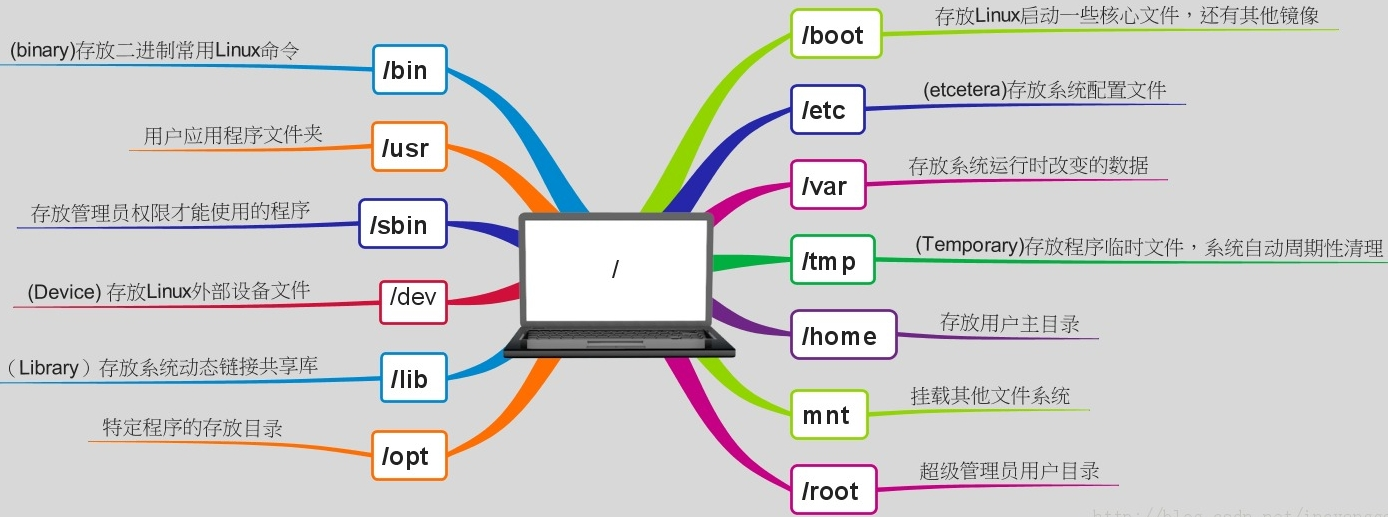
\includegraphics[width=12cm]{c3.filesystem.01.jpg}
  \end{figure}
  \pause
  \begin{block}{全称/助记}
    bin: binary; dev: device; lib: library; mnt: mount; proc: process;\\
  etc: etcetera => Extended Tool Chest, Editable Text Configuration;\\
  opt: optional; sbin: system binary; srv: service; tmp: temporary;\\
  usr: user => User System/Software Resources; var: variable.
\end{block}
\end{frame}

\begin{frame}
  \frametitle{文件系统 | 基础 | 目录结构 | \alert{基本目录} | 详解(1/2)}
  \begin{table}
    \centering
    \rowcolors[]{1}{blue!20}{blue!10}
    \begin{tabular}{ll}
      \hline
      \rowcolor{blue!50}目录 & 内容\\
      \hline
      / & 根目录\\
      /bin & 基本程序\\
      /boot & 启动系统时所需的文件\\
      /dev & 设备文件\\
      /etc & 配置文件\\
      /home & 用户的home目录\\
      /lib & 基本共享库,内核模块\\
      /lost+found & 由fsck恢复的受损文件\\
      /media & 可移动介质的挂载点\\
      /mnt & 不能挂载在其他位置上的固定介质的挂载点\\
      \hline
    \end{tabular}
  \end{table}
\end{frame}

\begin{frame}
  \frametitle{文件系统 | 基础 | 目录结构 | \alert{基本目录} | 详解(2/2)}
  \begin{table}
    \centering
    \rowcolors[]{1}{blue!20}{blue!10}
    \begin{tabular}{ll}
      \hline
      \rowcolor{blue!50}目录 & 内容\\
      \hline
      /opt & 第三方应用程序(“可选软件”)\\
      /proc & proc文件\\
      /root & 根用户(超级用户)的home目录\\
      /sbin & 由超级用户运行的基本系统管理程序\\
      /srv & 本地系统所提供服务的数据\\
      /tmp & 临时文件\\
      /usr & 静态数据使用的辅助文件系统\\
      /var & 可变数据使用的辅助文件系统\\
      \hline
    \end{tabular}
  \end{table}
\end{frame}

\begin{frame}
  \frametitle{文件系统 | 基础 | 目录结构 | 基本目录}
  \begin{description}
    \item[/boot] 内核文件及自举程序文件保存位置
    \item[/dev] 存放设备文件
    \item[/etc] 系统配置文件
    \item[/home] 用户默认家目录
    \item[/lib] 存放系统程序运行所需的共享库
    \item[/lost+found] 存放一些系统出错的检查结果
    \item[/mnt] 临时文件系统的安装点
    \item[/proc] 虚拟文件系统,存放当前进程信息
    \item[/tmp] 存放临时文件
    \item[/usr] 存放所有命令、库、手册页等
    \item[/usr/bin,/bin] 存放所有用户可以执行的命令
    \item[/usr/sbin,/sbin] 存放只有root可以执行的命令
    \item[/var] 包含经常发生变动的文件,如邮件、日志文件、计划任务等
  \end{description}
\end{frame}

\begin{frame}
  \frametitle{文件系统 | 基础 | 目录结构 | 基本目录}
  \begin{figure}
    \centering
    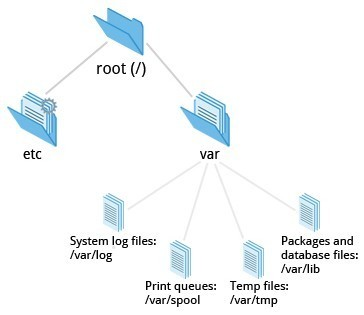
\includegraphics[width=6cm]{c3.etc.var.jpg}
    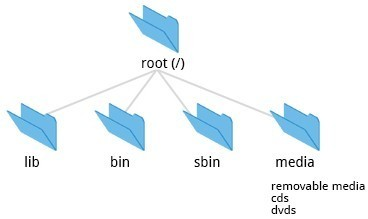
\includegraphics[width=6cm]{c3.lib.media.jpg}
  \end{figure}
\end{frame}

\begin{frame}
  \frametitle{文件系统 | 基础 | 目录结构 | 基本目录 | \alert{/usr}}
  \begin{table}
    \centering
    \rowcolors[]{1}{blue!20}{blue!10}
    \begin{tabular}{ll}
      \hline
      \rowcolor{blue!50}目录 & 内容\\
      \hline
      /usr/bin & 非基本程序(大多数用户程序)\\
      /usr/games & 游戏等娱乐和教育程序\\
      /usr/include & C程序的头文件\\
      /usr/lib & 非基本共享库\\
      /usr/local & 本地安装程序\\
      /usr/sbin & 由超级用户运行的非基本系统管理程序\\
      /usr/share & 共享系统数据\\
      /usr/src & 源代码(只用于参考)\\
      \hline
    \end{tabular}
  \end{table}
\end{frame}

\begin{frame}
  \frametitle{文件系统 | 基础 | 目录结构 | 基本目录 | /usr}
  \begin{figure}
    \centering
    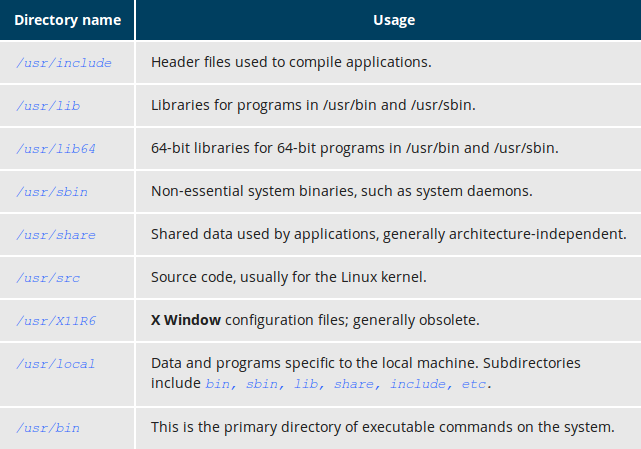
\includegraphics[width=10.5cm]{c3.usr.png}
  \end{figure}
\end{frame}

\begin{frame}
  \frametitle{文件系统 | 基础 | 目录结构 | 基本目录 | 程序目录}
  \begin{description}
    \item[/] 存放系统程序,也就是AT\&T开发的Unix程序
    \item[/usr] 存放Unix系统商(比如IBM和HP)开发的程序
    \item[/usr/local] 存放用户自己安装的程序
    \item[/opt] 在某些系统,用于存放第三方厂商开发的程序,所以取名为option,意为“选装”
  \end{description}
\end{frame}

\subsection{路径}
\begin{frame}[fragile]
  \frametitle{文件系统 | 基础 | \alert{路径}}
  \begin{block}{绝对 vs. 相对}
    \begin{itemize}
      \item 绝对路径(Absolute Path):文件在文件系统中的精确位置,总是起始于root(/)
      \item 相对路径(Relative Path):相对于用户当前位置的一个文件或目录的位置
    \end{itemize}
  \end{block}
  \pause
  \begin{block}{相对路径}
    \begin{itemize}
      \item \verb|.|:当前目录
      \item \verb|..|:上一层目录
      \item \verb|~|:当前用户的家目录(Home Directory)
      \item \verb|-|:上一个工作目录
    \end{itemize}
  \end{block}
\end{frame}

\begin{frame}[fragile]
  \frametitle{文件系统 | 基础 | 路径 | 绝对 vs. 相对}
  \begin{figure}
    \centering
    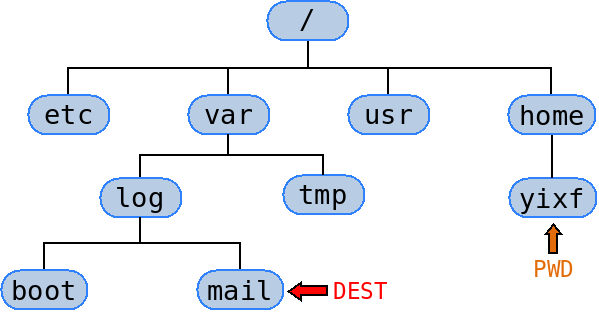
\includegraphics[width=9cm]{c3.path.png}
  \end{figure}
  \pause
  \begin{block}{绝对 vs. 相对}
    %\begin{itemize}[<+-|alert@+>]
    \begin{itemize}[<+->]
      \item 绝对路径:\verb|/var/log/mail|;精确 vs. 冗长
      \item 相对路径:\verb|../../var/log/mail|;(多数时候)简短 vs. 隐患
    \end{itemize}
  \end{block}
\end{frame}

\begin{frame}[fragile]
  \frametitle{文件系统 | 基础 | \alert{补充}}
  %\begin{itemize}[<+-|alert@+>]
  \begin{itemize}[<+->]
    \item 一切都源于根目录(\verb|/|)
    \item 文件名除了\verb|/|之外,所有的字符都合法
    \item 有些字符最好不用,如空格符、制表符、退格符和\verb|@#$&()-|等字符
    \item 避免使用\verb|.|作为普通文件名的第一个字符(隐藏文件)
    \item 大小写敏感,Linux是区分大小写的操作系统
    \item real\_file、Real\_file、REAL\_FILE是三个不同的文件名
    \item 按惯例文件名都是小写的
  \end{itemize}
\end{frame}

\section{文件系统导航}
\begin{frame}
  \frametitle{文件系统 | 导航}
  \begin{columns}
    \pause
    \column[t]{0.3\textwidth}
    \begin{block}{目录}
      \begin{itemize}
        \item 定位
        \item 切换
        \item 列出
        \item 创建
        \item 删除
        \item 树图
        \item \ldots
      \end{itemize}
    \end{block}
    \pause
    \column[t]{0.3\textwidth}
    \begin{block}{文件}
      \begin{itemize}
        \item 查看
        \item 识别
	\item 状态
        \item 创建
        \item 复制
        \item 移动
        \item 重命名
        \item 删除
        \item \ldots
      \end{itemize}
    \end{block}
    \pause
    \column[t]{0.3\textwidth}
    \begin{block}{管理}
      \begin{itemize}
        \item 查找
        \item 空间
        \item 大小
        \item \ldots
      \end{itemize}
    \end{block}
  \end{columns}
\end{frame}

\subsection{目录操作}
\begin{frame}
  \frametitle{文件系统 | 导航 | \alert{目录}}
  \begin{table}
    \centering
    \rowcolors[]{1}{blue!20}{blue!10}
    \begin{tabular}{ccl}
      \hline
      \rowcolor{blue!50}命令 & 助记 & 说明\\
      \hline
      pwd & Print Work Directory & 显示用户的当前目录\\
      ls & LiSt & 列出指定目录的内容\\
      cd & Change Directory & 转到指定的目录\\
      mkdir & MaKe DIRectory & 创建指定的目录\\
      rmdir & ReMove DIRectory & 删除空目录\\
      tree & --- & 以树状图列出目录的内容结构\\
      \hline
    \end{tabular}
  \end{table}
\end{frame}

\subsection{文件操作}
\begin{frame}
  \frametitle{文件系统 | 导航 | \alert{文件}}
  \begin{table}
    \centering
    \rowcolors[]{1}{blue!20}{blue!10}
    \begin{tabularx}{0.9\textwidth}{ccX}
      \hline
      \rowcolor{blue!50}命令 & 助记 & 说明\\
      \hline
      file & --- & 识别文件类型(二进制、文本等)\\
      cat & conCATenate & 显示一个文件\\
      touch & --- & 创建一个空文件或者修改一个现有文件的属性\\
      stat & STATus & 查看文件的详细属性/状态\\
      cp & CoPy & 把一个文件/目录复制到指定位置\\
      mv & MoVe & 移动文件/目录的位置或重命名一个文件/目录\\
      rm & ReMove & 删除文件\\
      head & --- & 显示文件的开始部分\\
      tail & --- & 显示文件的结尾部分\\
      more & --- & 从头到尾浏览一个文件\\
      less & --- & 从开头或结尾开始浏览整个文件\\
      %ln & LiNk & 创建链接\\
      %chmod & CHange file MODe & 改变文件属性\\
      %wc & Word Count & 计算文件行、字(符)数\\
      %mount & --- & 挂载文件系统\\
      \hline
    \end{tabularx}
  \end{table}
\end{frame}

\subsection{文件系统管理}
\begin{frame}
  \frametitle{文件系统 | 导航 | \alert{管理}}
  \begin{table}
    \centering
    \rowcolors[]{1}{blue!20}{blue!10}
    \begin{tabularx}{0.9\textwidth}{ccX}
      \hline
      \rowcolor{blue!50}命令 & 助记 & 说明\\
      \hline
      which & --- & 如果文件位于用户的PATH内,则显示文件位置\\
      whereis & --- & 显示文件的位置\\
      find & --- & 查找文件/目录\\
      df & Disk Free & 显示磁盘空间的使用情况\\
      du & Disk Usage & 显示目录空间占用情况\\
      \hline
    \end{tabularx}
  \end{table}
\end{frame}

\subsection{命令详解}
\begin{frame}
  \frametitle{文件系统 | 导航 | 命令详解 | cp}
  \begin{block}{选项}
    \begin{itemize}
      \item -p:Preserve,保持目录和文件的属性
      \item -R:Recursive,递归
      \item -u:Update,增量备份
    \end{itemize}
  \end{block}
  \pause
  \begin{block}{cp妙用:备份目录}
    cp\quad -Rpu\quad 待备份目录\quad 目标目录
  \end{block}
\end{frame}

\begin{frame}[fragile]
  \frametitle{文件系统 | 导航 | 命令详解 | cd}
  \begin{block}{\alert{cd}}
    \begin{itemize}
      \item \verb|cd|:返回家目录
      \item \verb|cd ~|:返回家目录
      \item \verb|cd ..|:返回上一层目录
    \end{itemize}
  \end{block}
  \pause
  \begin{block}{which vs. whereis}
    \begin{itemize}
      \item which:只在用户的PATH所指定的文件中查找
      \item whereis:在系统的所有目录中定位要查找的命令
    \end{itemize}
  \end{block}
  \pause
  \begin{block}{find}
    \verb|find /usr/share -name lostfile -print|
  \end{block}
\end{frame}

\begin{frame}[fragile]
  \frametitle{文件系统 | 导航 | 命令详解 | \alert{ls}}
  %\begin{itemize}[<+-|alert@+>]
  \begin{itemize}[<+->]
    \item \verb|ls|:列出用户有权访问的任何目录的内容
    \item \verb|ls -i|(Inode):显示文件的inode信息
    \item \verb|ls -a|(All):显示所有的文件和目录,包括隐藏的文件和目录
    \item 在文件名的前面加一个\verb|.|(英文句号)可以隐藏该文件或目录
    \item \verb|ls -l|(Long):显示目录内容的相关扩展信息
  \end{itemize}
  \begin{figure}
    \centering
    \visible<5>{ 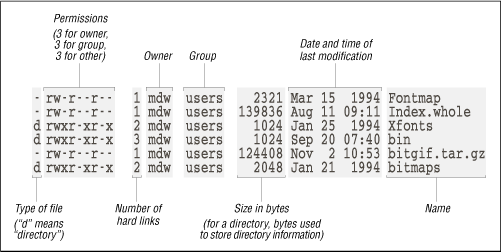
\includegraphics[width=10cm]{c3.ls.png} }
  \end{figure}
\end{frame}

\begin{frame}[fragile]
  \frametitle{文件系统 | 导航 | 命令详解 | cat}
  \begin{block}{cat vs. more vs. less}
    友好性:cat $\textless$ more $\textless$ less
  \end{block}
  \pause
  \begin{block}{\alert{head vs. tail}}
    \begin{itemize}
      \item 默认显示文件的前/后10行
      \item \verb|-n x|:指定查看文件的前/后x行
      \item \verb|tail -f|(Follow):监视文件内容的变化
    \end{itemize}
  \end{block}
\end{frame}

\begin{frame}[fragile]
  \frametitle{文件系统 | 导航 | 命令详解 | \alert{rm}}
  %\begin{itemize}[<+-|alert@+>]
  \begin{itemize}[<+->]
    \item \verb|rmdir|:只能删除空目录
    \item \verb|rm|:不能删除目录
    \item \verb|-f|(Force):强行删除文件
    \item \verb|-r|(Recursive):进入到目录中递归删除文件
    \item \verb|-fr|:删除目录及其子目录,\textcolor{red}{\textbf{谨慎使用}}
    \item \textcolor{red}{\textbf{切勿尝试}}:\verb|rm -rf /|,\verb|rm -rf *|
  \end{itemize}
\end{frame}

\begin{frame}[fragile]
  \frametitle{文件系统 | 导航 | 命令详解 | \alert{df}}
  \begin{figure}
    \centering
    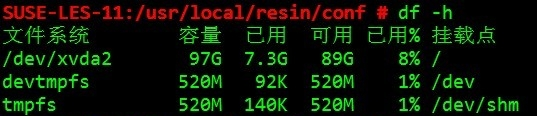
\includegraphics[width=10cm]{c3.df.01.jpg}\\
    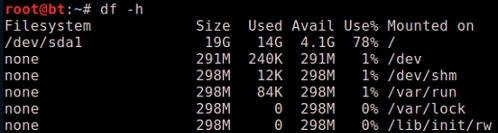
\includegraphics[width=10cm]{c3.df.02.jpg}
  \end{figure}
  \vspace{-0.5cm}
  \begin{block}{参数}
    \begin{itemize}
      \item \verb|df -h|,\verb|du -h|(Human-readable):K,M,G
      \item \verb|du -s|(Summarize):目录的总大小
    \end{itemize}
  \end{block}
\end{frame}

\section{文件类型}
\subsection{类型简介}
\begin{frame}
  \frametitle{文件系统 | 文件类型 | 简介}
  \begin{table}
    \centering
    \rowcolors[]{1}{blue!20}{blue!10}
    \begin{tabular}{cm{0.7\columnwidth}}
      \hline
      \rowcolor{blue!50}文件类型 & 说明\\
      \hline
      \alert{-} & 普通文件(文本文件、二进制可执行文件、硬链接)\\
      \alert{d} & 目录文件\\
      \alert{l(小写L)} & 符号链接文件\\
      b & 块设备文件(块输入/输出设备文件,如存储设备)\\
      %c & 字符设备文件(原始输入/输出设备文件,将数据作为字节流处理,如Terminal)\\
      c & 字符设备文件(原始输入/输出设备文件,将数据作为字节流处理,如Terminal)\\
      p & 命令管道(一种进程间通信的机制)\\
      s & 套接字(用于进程间通信)\\
      \hline
    \end{tabular}
  \end{table}
\end{frame}

\subsection{链接}
\begin{frame}
  \frametitle{文件系统 | 文件类型 | 链接 | inode}
  %\begin{itemize}[<+-|alert@+>]
  \begin{itemize}[<+->]
    \item 在Linux中,每一个文件都有一个相关联的数字:inode
    \item Linux使用inode而不是文件名来引用文件
    \item 在一个分区中,inode是唯一的
    \item 不同分区内的文件可以有相同的inode
  \end{itemize}
  \begin{figure}
    \centering
    \visible<5>{ 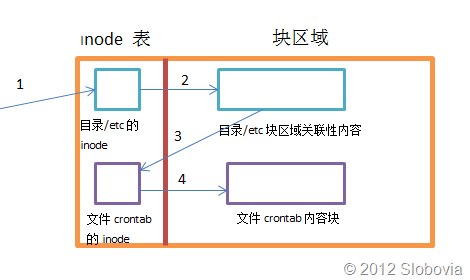
\includegraphics[width=10cm]{c3.inode.12.png} }
  \end{figure}
\end{frame}

\begin{frame}
  \frametitle{文件系统 | 文件类型 | \alert{链接}}
  \begin{block}{硬链接(Hard Link)}
    %\begin{itemize}[<+-|alert@+>]
    \begin{itemize}[<+->]
      \item 硬链接与原文件具有相同的inode,两者本质上没有区别
      \item 对硬链接的修改会反映到原文件上,反之亦然
      \item 如果删除硬链接,原文件照样正常使用,反之亦然
      \item 不能跨越文件系统,“等同于”不占空间的复制+同步更新
      \item 只能对文件建立硬链接,而不能对目录建立硬链接
    \end{itemize}
  \end{block}
  \pause
  \begin{block}{软链接(Soft Link,符号链接,Symbolic Link)}
    %\begin{itemize}[<+-|alert@+>]
    \begin{itemize}[<+->]
      \item 能够跨越文件系统,相当于Windows中的快捷方式
      \item 软链接具有唯一的inode,内部保存的是原文件的路径地址
      \item 如果打开并修改软链接,原文件也会随之改变
      \item 如果删除软链接,原文件并不会受到影响
      \item 如果删除原文件,软链接将失效
    \end{itemize}
  \end{block}
\end{frame}

\begin{frame}
  \frametitle{文件系统 | 文件类型 | 链接}
  \begin{figure}
    \centering
    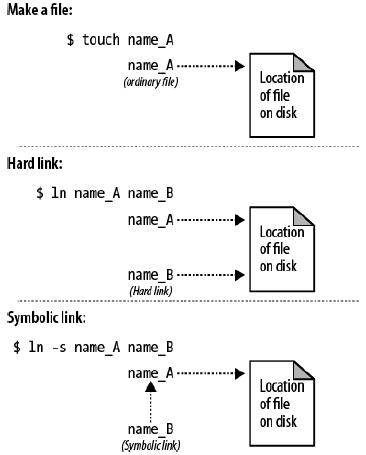
\includegraphics[width=6cm]{c3.ln.png}
  \end{figure}
\end{frame}

\begin{frame}
  \frametitle{文件系统 | 文件类型 | 链接 | \alert{比较}}
  \begin{table}
    \centering
    \rowcolors[]{1}{blue!20}{blue!10}
    \begin{tabularx}{0.94\textwidth}{ccc}
      \hline
      \rowcolor{blue!50}项目 & 硬链接 & 软链接\\
      \hline
      语法(LiNk) & ln source hardlink & ln -s source softlink\\
      本质 & 与原文件没区别 & 保存原文件的路径\\
      inode & 与原文件相同 & 与原文件不同,唯一\\
      类比 & 不占空间的复制+同步更新 & 快捷方式\\
      文件系统 & 不能跨越 & 能跨越\\
      删除原文件 & 不受影响 & 失效\\
      使用对象 & 文件 & 文件和目录\\
      \hline
      修改链接 & \multicolumn{2}{c}{原文件随之改变}\\
      删除链接 & \multicolumn{2}{c}{原文件不受影响}\\
      \hline
    \end{tabularx}
  \end{table}
\end{frame}

\begin{frame}
  \frametitle{文件系统 | 文件类型 | 链接 | 用途}
  \begin{itemize}
    \item 为命令、程序或文件取别名
    \item 创建不占存储空间的文件副本
    \item 为文件创建方便的快捷方式
    \item 对文件进行分组
  \end{itemize}
\end{frame}

\section{文件和目录权限}
\subsection{权限简介}
\begin{frame}
  \frametitle{文件系统 | 权限 | \alert{简介}}
  \begin{figure}
    \centering
    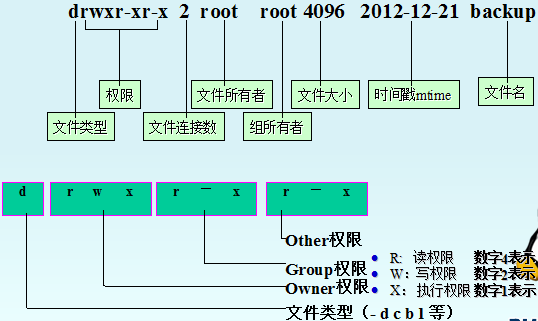
\includegraphics[width=11cm]{c3.permission.01.png}
  \end{figure}
\end{frame}

\begin{frame}
  \frametitle{文件系统 | 权限 | \alert{简介}}
  \begin{figure}
    \centering
    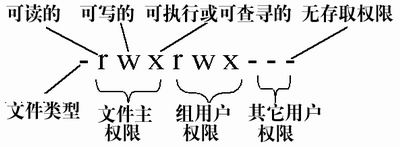
\includegraphics[width=8cm]{c3.ugo.01.png}
  \end{figure}
  \begin{table}
    \centering
    \rowcolors[]{1}{blue!20}{blue!10}
    \begin{tabular}{ccl}
      \hline
      \rowcolor{blue!50}字符位置 & 含义 & 助记\\
      \hline
      2~4 & 文件所有者 & user\\
      5~7 & 文件所属组 & group\\
      8~10 & 其他任何人 & others\\
      \hline
    \end{tabular}
  \end{table}
\end{frame}

\begin{frame}
  \frametitle{文件系统 | 权限 | 简介 | \alert{基本类型}}
  \begin{table}
    \centering
    \rowcolors[]{1}{blue!20}{blue!10}
    \begin{tabularx}{\textwidth}{cccXX}
      \hline
      \rowcolor{blue!50}字符 & 助记 & 权限 & 对文件 & 对目录\\
      \hline
      r & Read & 读 & 查看文件内容【cat】 & 读取/列出目录或子目录内容【ls】\\
      w & Write & 写 & 修改文件内容(添加文本或删除文件)【vim】 & 在目录中创建、修改、删除文件或子目录【touch】\\
      x & eXecute & 执行 & 执行/运行文件【sh】 & 进入目录搜索【cd】\\
      - & - & - & 无 & 无\\
      \hline
    \end{tabularx}
  \end{table}
  \centering
  注意:目录必须具有x权限,否则无法进入并查看其内容!
\end{frame}

\subsection{修改权限}
\begin{frame}
  \frametitle{文件系统 | 权限 | \alert{修改}}
  \begin{block}{修改权限}
    chmod(CHange MODe)
  \end{block}
  \pause
  \begin{block}{两种方式}
    \begin{enumerate}
      \item 符号模式:容易理解
        \begin{itemize}
          \item 用户:u, g, o, a
          \item 操作:+, -, =
	  \item 权限:r, w, x
	  %\item 权限:r, w, x, \textcolor{gray}{-}
        \end{itemize}
      \item 绝对模式:更加高效
        \begin{itemize}
          \item 0, 1, 2, 4
          \item $3 = 1 + 2$
          \item $5 = 1 + 4$
          \item $6 = 2 + 4$
          \item $7 = 1 + 2 + 4$
        \end{itemize}
    \end{enumerate}
  \end{block}
\end{frame}

\begin{frame}[fragile]
  \frametitle{文件系统 | 权限 | 修改 | \alert{符号模式}}
  \begin{columns}
    \column[t]{0.35\textwidth}
    \begin{block}{用户}
      \begin{itemize}
        \item u:User,用户
        \item g:Group,组
        \item o:Other,其他人
        \item a:All,所有人
      \end{itemize}
    \end{block}
    \pause
    \column[t]{0.2\textwidth}
    \begin{block}{操作}
      \begin{itemize}
        \item +:添加
        \item -:删除
        \item =:指定
      \end{itemize}
    \end{block}
    \pause
    \column[t]{0.35\textwidth}
    \begin{block}{权限}
      \begin{itemize}
        \item r:Read,读
        \item w:Write,写
        \item x:eXecute,执行
	%\item \textcolor{gray}{-:无}
        %\item -:无
      \end{itemize}
    \end{block}
  \end{columns}
  \pause
  \begin{block}{实例}
    \begin{itemize}
      \item \verb|chmod u-x testfile|
      %\item \verb|chmod g=r-x testfile|
      \item \verb|chmod g=rx testfile|
      \item \verb|chmod o+wx testfile|
      \item \verb|chmod uo+x,g-w testfile|
      %\item \verb|chmod u-x,g=r-x,o+wx testfile|
      \item \verb|chmod u-x,g=rx,o+wx testfile|
    \end{itemize}
  \end{block}
\end{frame}

\begin{frame}[fragile]
  \frametitle{文件系统 | 权限 | 修改 | \alert{绝对模式}}
  \begin{table}
    \centering
    \rowcolors[]{1}{blue!20}{blue!10}
    \begin{tabular}{ccl}
      \hline
      \rowcolor{blue!50}数字 & 符号 & 权限\\
      \hline
      0 & \verb|---| & 无权限\\
      1 & \verb|--x| & 可执行\\
      2 & \verb|-w-| & 可写\\
      3 & \verb|-wx| & 可写、可执行(2+1)\\
      4 & \verb|r--| & 可读\\
      5 & \verb|r-x| & 可读、可执行(4+1)\\
      6 & \verb|rw-| & 可读、可写(4+2)\\
      7 & \verb|rwx| & 可读、可写、可执行(4+2+1)\\
      \hline
    \end{tabular}
  \end{table}
  \pause
  \begin{block}{实例}
    \begin{itemize}
      \item \verb|chmod 740 testfile|
      \item \verb|chmod 755 testfile|
    \end{itemize}
  \end{block}
\end{frame}

\subsection{特殊权限}
\begin{frame}[fragile]
  \frametitle{\textcolor{gray}{特殊权限 | SetUID}}
  \begin{block}{SetUID:Set User ID,设置用户标识}
    当一个可执行程序(一般为一个命令)具有SetUID权限,用户执行这个程序时,将以这个程序的所有者的身份执行。
  \end{block}
  \pause
  \begin{block}{设置SetUID}
    \begin{itemize}
      \item 设置:\verb|chmod u+s FILE|,\verb|chmod 4755 FILE|(SetUID=4000)
      \item 取消:\verb|chmod u-s FILE|,\verb|chmod 755 FILE|
      \item 查看:\verb|-rwsr-xr-x 1 root root ... /usr/bin/passwd|
      \item 查找:\verb|find / -perm -4000|
    \end{itemize}
  \end{block}
  \pause
  \begin{block}{注意事项}
    将命令设置成SetUID是一件很危险的事情!它可以让一个用户瞬间变成超级用户、使系统不断重启、使用户不需要密码就可以登录……比如将vi设置成SetUID,则它可以编辑并保存系统中所有的文件,甚至是系统配置文件!
  \end{block}
\end{frame}

\begin{frame}[fragile]
  \frametitle{\textcolor{gray}{特殊权限 | SetGID}}
  \begin{block}{SetGID:Set Group ID}
    当一个可执行程序(一般为一个命令)具有SetGID权限,用户执行这个程序时,将以这个程序所属组的身份执行。
  \end{block}
  \pause
  \begin{block}{设置SetGID}
    \begin{itemize}
      \item 设置:\verb|chmod g+s FILE|,\verb|chmod 2755 FILE|(SetGID=2000)
      \item 取消:\verb|chmod g-s FILE|,\verb|chmod 755 FILE|
      \item 查看:\verb|drwxr-s--- 2 root dip ... /etc/chatscripts/|
      \item 查找:\verb|find / -perm -2000|
      \item 同时设置SetUID和SetGID:\verb|chmod 6755 FILE|
    \end{itemize}
  \end{block}
\end{frame}

\begin{frame}[fragile]
  \frametitle{\textcolor{gray}{特殊权限 | 粘着位}}
  \begin{block}{粘着位(Sticky Bit)}
    如果一个权限为777的目录,被设置了粘着位,每个用户都可以在这个目录里面创建文件,但是只可以删除所有者是自己的文件。
  \end{block}
  \pause
  \begin{block}{设置粘着位}
    \begin{itemize}
      \item 设置:\verb|chmod o+t DIR|,\verb|chmod +t DIR|,\verb|chmod 1777 DIR|(粘着位=1000)
      \item 取消:\verb|chmod o-t DIR|,\verb|chmod -t DIR|,\verb|chmod 777 DIR|
      \item 查看:\verb|drwxrwxrwt 15 root root ... /tmp|
      \item 查找:\verb|find / -perm -1000|
    \end{itemize}
  \end{block}
  \pause
  \begin{block}{注意事项}
    设定粘着位的条件是文件必须具有777的权限,否则没有意义。
  \end{block}
\end{frame}

\begin{frame}[fragile]
  \frametitle{\textcolor{gray}{特殊权限 | 总结}}
  The \verb|chmod| command can be used to set or unset with the following values as a \textbf{prefix} to the normal three numeric privileges:
  \begin{table}
    \centering
    \rowcolors[]{1}{blue!20}{blue!10}
    \begin{tabular}{cl}
      \hline
      \rowcolor{blue!50}Value & Explanation\\
      \hline
      0 & SetUID, SetGID, sticky bits are unset\\
      1 & sticky bit is in place\\
      2 & SetGID bit is in place\\ 
      3 & SetGID and sticky bits are in place\\
      4 & SetUID bit is in place\\
      5 & SetUID and sticky bits are in place\\
      6 & SetUID and SetGID bits are on\\
      7 & SetUID, SetGID, sticky bits are activated\\
      \hline
    \end{tabular}
  \end{table}
\end{frame}

\begin{frame}[fragile]
  \frametitle{\textcolor{gray}{特殊权限 | 补充}}
  \begin{table}
    \centering
    \rowcolors[]{1}{blue!20}{blue!10}
    \begin{tabular}{cl}
      \hline
      \rowcolor{blue!50} Permissions & Meaning\\
      \hline
      \verb|--S------| & SetUID is set, but user (owner) execute is not set.\\
      \verb|--s------| & SetUID and user execute are both set.\\
      \verb|-----S---| & SetGID is set, but group execute is not set.\\
      \verb|-----s---| & SetGID and group execute are both set.\\
      \verb|--------T| & Sticky bit is set, bot other execute is not set.\\
      \verb|--------t| & Sticky bit and other execute are both set.\\
      \hline
    \end{tabular}
  \end{table}
\end{frame}

\section{挂载文件系统}
\begin{frame}[fragile]
  \frametitle{文件系统 | 挂载 | mount }
  \begin{figure}
    \centering
    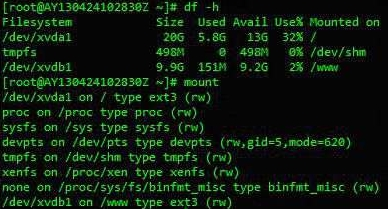
\includegraphics[width=9cm]{c3.mount.jpg}
  \end{figure}
  \pause
  \vspace{-0.3cm}
  \begin{block}{\alert{语法}}
    \begin{itemize}
      \item \verb|mount -t FILE.SYSTEM.TYPE DEVICE DIRECTORY|
      \item \verb|mount -t iso9660 /dev/cdrom /mnt/cdrom|
      \item \verb|umount DEVICE.TO.UNMOUNT|
      \item \verb|umount /dev/cdrom|
    \end{itemize}
  \end{block}
\end{frame}

\section{回顾与总结}
\subsection{总结}
\begin{frame}
  \frametitle{文件系统 | 总结}
  \begin{block}{知识点}
    \begin{itemize}
      \item Linux的文件系统:目录结构,主要的基本目录
      \item Linux中的路径:绝对路径和相对路径
      \item 文件系统导航的常见命令
      \item Linux中的文件类型:常见类型,硬链接和软链接
      \item Linux中的权限:文件和目录的权限,符号模式和绝对模式
      \item 文件系统的挂载与卸载
    \end{itemize}
  \end{block}
  \begin{block}{技能}
    \begin{itemize}
      \item 在命令行中进行文件系统的导航
      \item 在命令行中创建硬链接和软链接
      \item 在命令行中修改文件的权限
      \item 在命令行中挂载、卸载文件系统
    \end{itemize}
  \end{block}
\end{frame}

\subsection{思考题}
\begin{frame}
  \frametitle{文件系统 | 思考题}
  \begin{enumerate}
    \item 列举Linux中的基本目录并解释其功能。
    \item 举例说明绝对路径和相对路径的区别。
    \item 列举几个进行文件系统导航的命令。
    \item 解释ls -l输出结果中每一列的含义。
    \item 比较Linux中的硬链接和软链接。
    \item Linux中的权限包括几种,针对哪些用户?
    \item 文件和目录的rwx权限有何异同?
    \item 举例说明如何使用符号模式修改权限?
    \item 举例说明如何使用绝对模式修改权限?
  \end{enumerate}
\end{frame}

\begin{frame}
  \frametitle{下节预告}
  总结日常使用Windows过程中的基本操作:目录操作、文件操作、系统管理、压缩解压、关机重启、……
\end{frame}



\section*{Acknowledgements}
\begin{frame}
  \frametitle{Powered by}
  \begin{center}
    
\includegraphics[width=9cm]{power.png}
  \end{center}
\end{frame}

\end{document}

